The Table \ref{tab:bpm_table_noBase} presents the average heart rate by each participant on each scenes and they are plotted in the Figures \ref{fig:barplot_ecg_bpm_4_scene_blind} to \ref{fig:barplot_ecg_bpm_4_scene}.


\begin{table}[!htb]
\centering
\caption{ECG average BPM felled by the participants using the proposed methods [BPM].}
\label{tab:bpm_table_noBase}
\begin{tabular}{lllrrrrr}
\toprule
    &       &        &  Audio & \begin{tabular}[c]{@{}l@{}}Haptic\\ Belt\end{tabular} & \begin{tabular}[c]{@{}l@{}}Virtual\\ Cane\end{tabular} & Mixture \\
Part. & \begin{tabular}[c]{@{}l@{}}Visual\\ Condition\end{tabular} & Round &        &                                                       &                                                        &         \\
\midrule
001 & Sight & First &  71.23 &                                                 63.02 &                                                  64.85 &   58.77 \\
    &       & Return &  73.18 &                                                 61.18 &                                                  66.78 &   66.26 \\
001C & Blind & First &  60.71 &                                                 71.17 &                                                  59.07 &   68.24 \\
    &       & Return &  58.61 &                                                 66.22 &                                                  64.20 &   70.76 \\
002C & Blind & First &  38.67 &                                                 48.74 &                                                  46.89 &   52.23 \\
    &       & Return &  47.58 &                                                 58.97 &                                                  56.75 &   58.25 \\
003 & Sight & First &  63.47 &                                                 71.80 &                                                  70.90 &   72.76 \\
    &       & Return &  72.75 &                                                 71.23 &                                                  67.49 &   73.01 \\
003C & Blind & First &  69.89 &                                                 70.95 &                                                  69.41 &   66.94 \\
    &       & Return &  67.44 &                                                 69.68 &                                                  68.82 &   67.37 \\
004 & Sight & First &  66.85 &                                                 62.45 &                                                  65.94 &   67.86 \\
    &       & Return &  69.48 &                                                 65.65 &                                                  64.58 &   71.86 \\
004C & Blind & First &  73.55 &                                                 73.70 &                                                  71.94 &   74.03 \\
    &       & Return &  74.79 &                                                 74.02 &                                                  72.69 &   67.34 \\
005 & Sight & First &  71.34 &                                                 66.93 &                                                  66.46 &   67.06 \\
    &       & Return &  69.57 &                                                 65.97 &                                                  67.00 &   65.47 \\
\bottomrule
\end{tabular}
\end{table}



The Figures \ref{fig:barplot_ecg_bpm_4_scene_blind} show and increase between all methods, whilst the Figure \ref{fig:barplot_ecg_bpm_4_scene_sight} also presents a decrease in two methods. The Figure \ref{fig:barplot_ecg_bpm_4_scene} shows that in most methods, the average BPM of the sight users was slight higher than the blind users.

\begin{figure}[!htb]
    \centering
    \begin{minipage}{\textwidth}
        \centering
        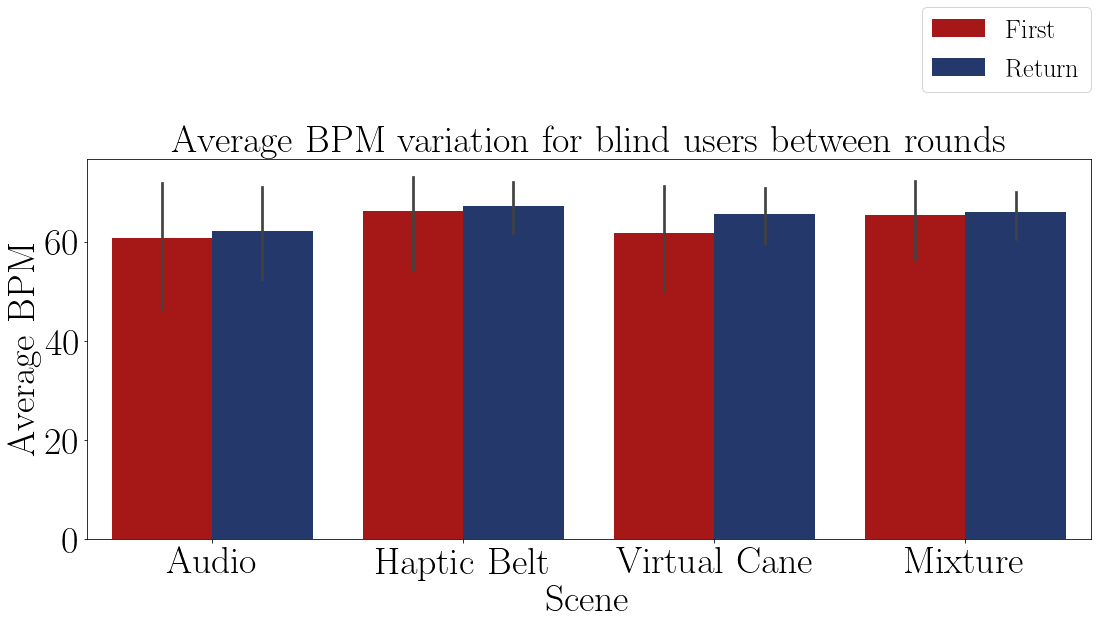
\includegraphics[width = 0.8\linewidth]{Resultados/ECG/Figuras/png/barplot_ecg_bpm_4_scene_blind.png}
        \caption{Barplot of the average BPM of the blind participants on each method and round.}
        \label{fig:barplot_ecg_bpm_4_scene_blind}
    \end{minipage}
    \begin{minipage}{\textwidth}
        \centering
        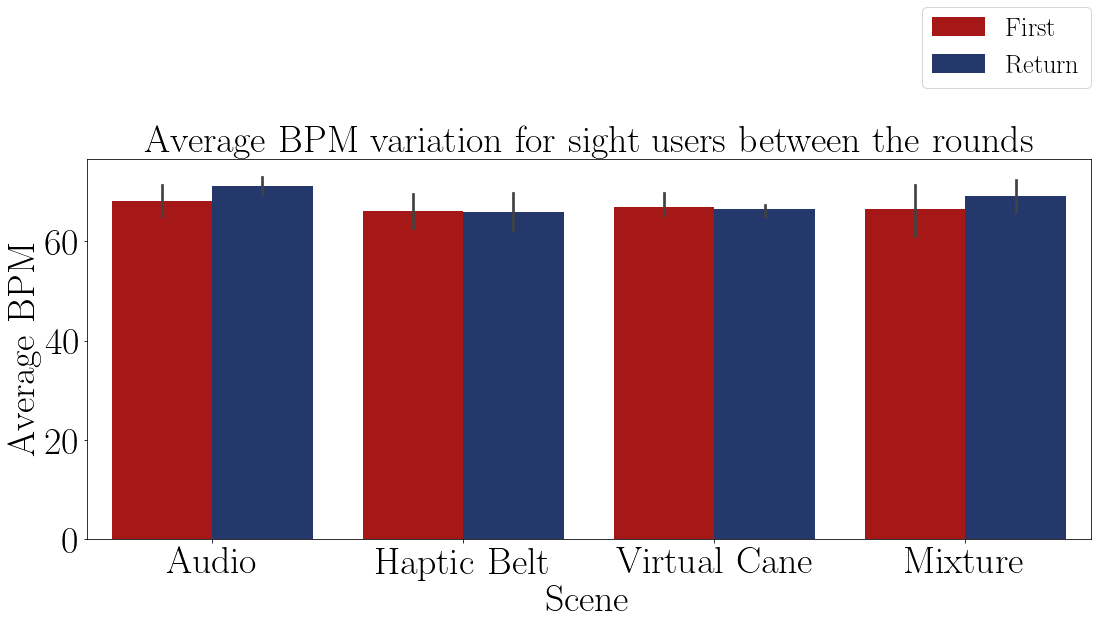
\includegraphics[width = 0.8\linewidth]{Resultados/ECG/Figuras/png/barplot_ecg_bpm_4_scene_sight.png}
        \caption{Barplot of the average BPM of the sight participants on each method and round.}
        \label{fig:barplot_ecg_bpm_4_scene_sight}
    \end{minipage}
\end{figure}
\begin{figure}[!htb]
    \centering
    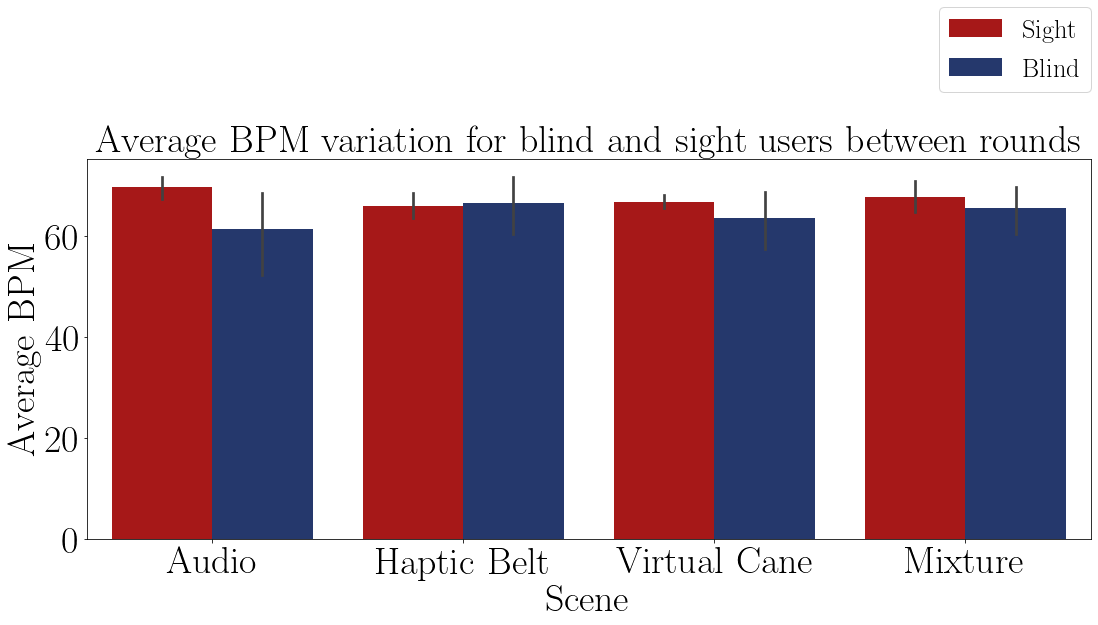
\includegraphics[width = 0.8\linewidth]{Resultados/ECG/Figuras/png/barplot_ecg_bpm_4_scene.png}
    \caption{Barplot of the average BPM of both participants on each method.}
    \label{fig:barplot_ecg_bpm_4_scene}
\end{figure}

The Figure \ref{fig:boxplot_ecg_bpm_4_scene} and \ref{fig:boxplot_ecg_bpm_4_rounds} presents a box plot with the average BPM of both groups by method and rounds in that order. These figures show the reaction of the sight user was very different from the blind users, in all methods and rounds.

\begin{figure}[!htb]
    \centering
    \begin{minipage}{0.45\textwidth}
        \centering
        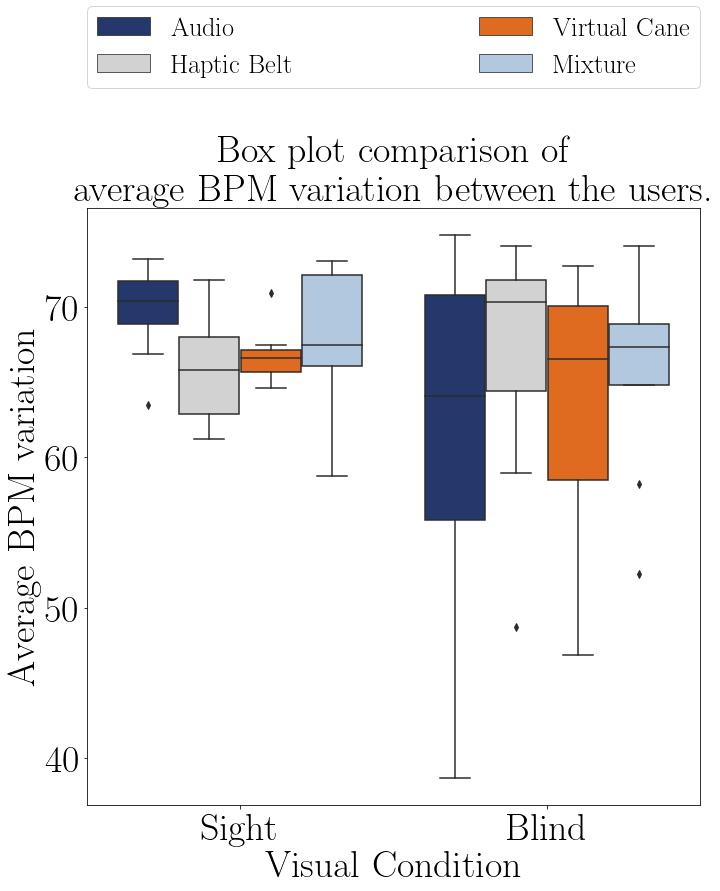
\includegraphics[width = 0.8\linewidth]{Resultados/ECG/Figuras/png/boxplot_ecg_bpm_4_scene.png}
        \caption{Boxplot of the average BPM of the participants grouped by method.}
        \label{fig:boxplot_ecg_bpm_4_scene}
    \end{minipage}
    \begin{minipage}{0.45\textwidth}
        \centering
        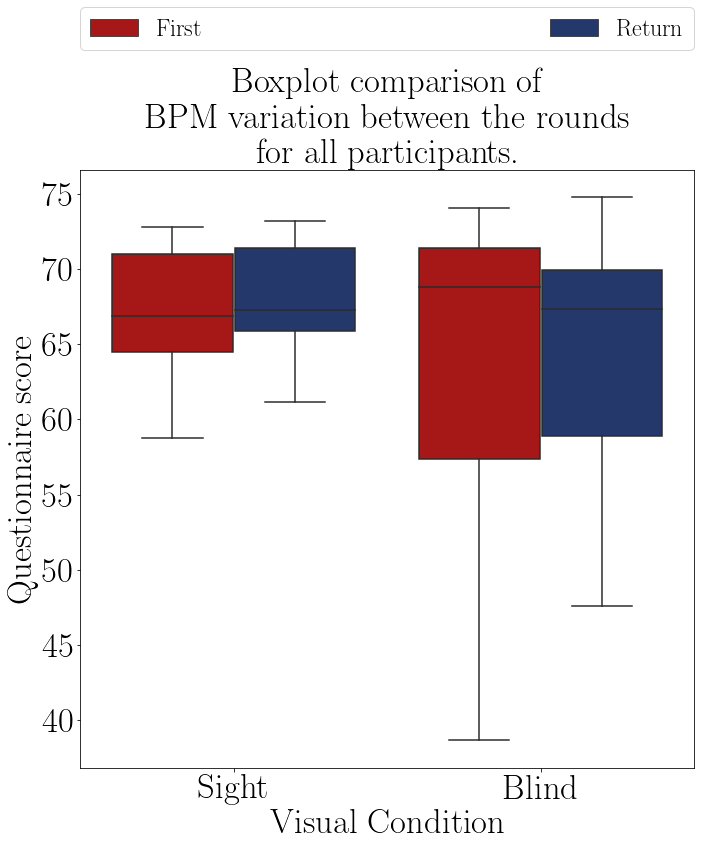
\includegraphics[width = 0.8\linewidth]{Resultados/ECG/Figuras/png/boxplot_ecg_bpm_4_rounds.png}
        \caption{Boxplot of the average BPM of the participants grouped by round.}
        \label{fig:boxplot_ecg_bpm_4_rounds}
    \end{minipage}
\end{figure}
 
The Table \ref{tab:bpm_average_group_noBase} shows the average heartrate of both samples and is possible to notice how the average score by the blind users was higher in every method, apart of the "Haptic Belt".


\begin{table}[!htb]
\centering
\caption{ECG average BPM for each method grouped by visual condition.}
\label{tab:bpm_average_group_noBase}
\begin{tabular}{lllrrrr}
\toprule
{} &  Audio & Haptic Belt & Virtual Cane & Mixture \\
Visual Condition &        &             &              &         \\
\midrule
Blind            &  61.40 &       66.68 &        63.72 &   65.65 \\
Sight            &  69.73 &       66.03 &        66.75 &   67.88 \\
\bottomrule
\end{tabular}
\end{table}



The Figures \ref{fig:qqplot_bpm_two_way_sight} and \ref{fig:residplot_bpm_two_way_sight} shows the distribution and variance of sighted participants of the Table \ref{tab:bpm_table_noBase}. These Figures shows that the data are normally distributed and that the methods have a similar variance.
The Table \ref{tab:blocanova_bpm_two_way_sight} shows the ANOVA test p-values of the average heartrate of the "sight" sample between the guidance methods and they show that the methods had an effect on the score.


\begin{table}[!htb]
\centering
\caption{Anova p-value for the BPM on each method for blinded users.}
\label{tab:blocanova_bpm_two_way_sight}
\begin{tabular}{lrrrrr}
\toprule
               Source &  Squared sum &  DOF & Squared average &     F & \begin{tabular}[c]{@{}l@{}}P-Value \\ $(F_{0} > F)$\end{tabular} \\
\midrule
Participants (Blocks) &       98.882 &    3 &          32.961 & 2.953 &                                                                  \\
         \    Methods &       62.635 &    3 &          20.878 & 1.870 &                                                            0.166 \\
          \    Rounds &       12.193 &    1 &          12.193 & 1.092 &                                                            0.308 \\
     \    Interaction &       19.626 &    3 &           6.542 & 0.586 &                                                            0.631 \\
   Experimental Error &      234.427 &   21 &          11.163 &       &                                                                  \\
                Total &      427.763 &   31 &                 &       &                                                                  \\
\bottomrule
\end{tabular}
\end{table}



\begin{figure}[!htb]
    \centering
    \begin{minipage}{0.45\textwidth}
        \centering
        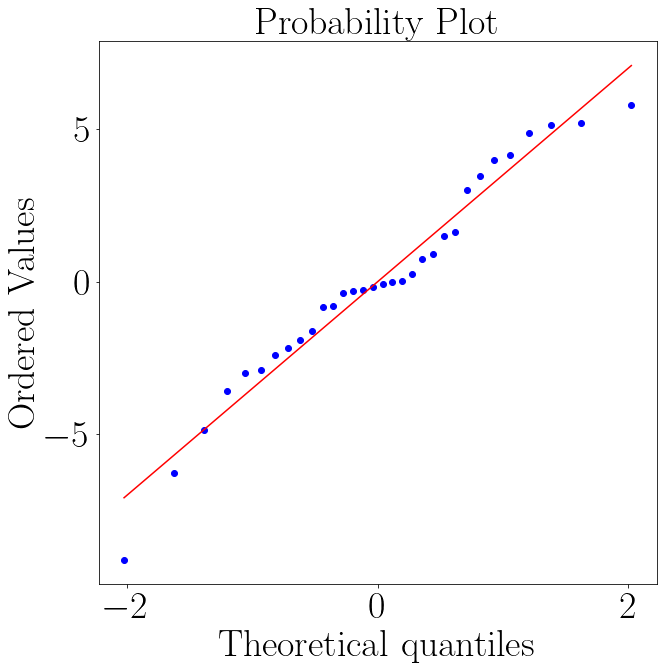
\includegraphics[width = 0.8\linewidth]{Resultados/ECG/Figuras/png/qqplot_bpm_two_way_sight.png}
        \caption{QQ plot of the BPM of the sight participants on each method.}
        \label{fig:qqplot_bpm_two_way_sight}
    \end{minipage}
    \begin{minipage}{0.45\textwidth}
        \centering
        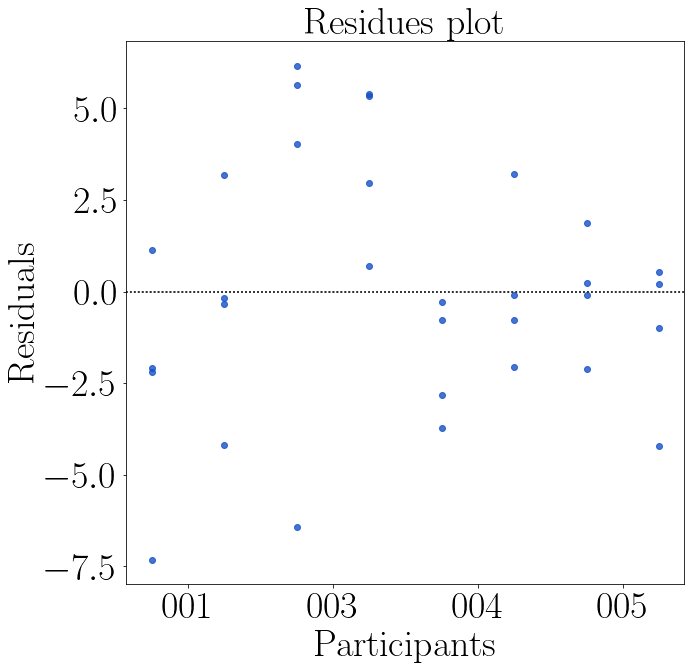
\includegraphics[width = 0.8\linewidth]{Resultados/ECG/Figuras/png/residplot_bpm_two_way_sight.png}
        \caption{Residual plot of the BPM score the sight participants on each method.}
        \label{fig:residplot_bpm_two_way_sight}
    \end{minipage}
\end{figure}

%
\begin{table}[!htb]
\centering
\caption{Cross validation p-value for the average BPM on each method for blinded users.}
\label{tab:lsd_bpm_two_way_sight}
\begin{tabular}{rclr}
\toprule
      \multicolumn{3}{c}{Method} &                          \multicolumn{2}{c}{Analysis} \\
\midrule
       Audio & $X$ & Haptic Belt &        $H_1 : \mu_{Audio} \ne \mu_{Haptic Belt}$ & ** \\
      Audio & $X$ & Virtual Cane &       $H_1 : \mu_{Audio} \ne \mu_{Virtual Cane}$ & ** \\
           Audio & $X$ & Mixture &            $H_1 : \mu_{Audio} \ne \mu_{Mixture}$ & ** \\
Haptic Belt & $X$ & Virtual Cane & $H_1 : \mu_{Haptic Belt} \ne \mu_{Virtual Cane}$ & ** \\
     Haptic Belt & $X$ & Mixture &      $H_1 : \mu_{Haptic Belt} \ne \mu_{Mixture}$ & ** \\
    Virtual Cane & $X$ & Mixture &     $H_1 : \mu_{Virtual Cane} \ne \mu_{Mixture}$ & ** \\
\bottomrule
\end{tabular}
\end{table}



%The Table \ref{tab:lsd_bpm_two_way_sight} presents the conclusion of a pairwise Fisher LSD test of the blind heart rate frequency variation between all the guidance methods and it shows that all methods had different effect on the heartrate.

According to the ANOVA test at Table \ref{tab:blocanova_bpm_two_way_sight} there was no effect of the methods neither the rounds or their interaction, despite the fact that the Figure \ref{fig:boxplot_ecg_bpm_4_scene} showed a big difference between the methods. So the methods did not influence the sighted user mental workload. The same conclusion was driven in the section \ref{subsubsec:results_ecg_1} in the BPM part.

\FloatBarrier